\documentclass[12pt,draftcls]{ucdavisthesis}

% PLEASE READ THE MANUAL - ucdavisthesis.pdf (in the package installation directory)

%%%%%%%%%%%%%%%%%%%%%%%%%%%%%%%%%%%%%%%%%%%%%%%%%%%%%%%%%%%%%%%%%%%%%%%%
%                                                                      %
%               LATEX COMMANDS FOR DOCUMENT SETUP                      %
%                                                                      %
%%%%%%%%%%%%%%%%%%%%%%%%%%%%%%%%%%%%%%%%%%%%%%%%%%%%%%%%%%%%%%%%%%%%%%%%

%\usepackage{bookmark}
\usepackage[us,nodayofweek,12hr]{datetime}
\usepackage{graphicx}
\usepackage{siunitx}
%\usepackage[square,comma,numbers,sort&compress]{natbib}
%\usepackage{hypernat}
% Other useful packages to try
\usepackage{amsmath}
\usepackage{amssymb}
%
% Different fonts to try (uncomment only fontenc and one font at a time)
% (you may need to install these first)
%\usepackage[T1]{fontenc} %enable fontenc package if using one of the fonts below
%\usepackage[adobe-utopia]{mathdesign}
%\usepackage{tgschola}
%\usepackage{tgbonum}
%\usepackage{tgpagella}
%\usepackage{tgtermes}
%\usepackage{fourier}
%\usepackage{fouriernc}
%\usepackage{kmath,kerkis}
%\usepackage{kpfonts}
%\usepackage[urw-garamond]{mathdesign}
%\usepackage[bitstream-charter]{mathdesign}
%\usepackage[sc]{mathpazo}
%\usepackage{mathptmx}
%\usepackage[varg]{txfonts}
%packages for CMS symbols
\usepackage{xspace}
\usepackage{ptdr-definitions}
\hyphenation{dis-ser-ta-tion blue-print man-u-script pre-par-ing} %add hyphenation rules for words TeX doesn't know


%\renewcommand{\rightmark}{\scriptsize A University of California Davis\ldots \hfill Rev.~\#1.0 \quad Compiled: \currenttime, \today}
% a fancier running header that can be used with draftcls options

%%%%%%%%%%%%%%%%%%%%%%%%%%%%%%%%%%%%%%%%%%%%%%%%%%%%%%%%%%%%%%%%%%%%%%%%
%                                                                      %
%        DOCUMENT SETUP AND INFORMATION FOR PRELIMINARY PAGES          %
%                                                                      %
%%%%%%%%%%%%%%%%%%%%%%%%%%%%%%%%%%%%%%%%%%%%%%%%%%%%%%%%%%%%%%%%%%%%%%%%

%\title          {A University of California Davis\\
%                 Dissertation/Thesis LaTeX Class File}
\title          {Search in Tau Final States for Higgs Decays to New Light Scalars\\
                 or Pseudoscalars in pp Collisions at $\sqrt{s} =$ 8 TeV}
%Exact title of your thesis. Indicate italics where necessary by underlining or using italics. Please capitalize the first letter of each word that would normally be capitalized in a title.

\author         {Francesca Shun-Ning Annarosa Ricci-Tam}
%Your full name as it appears on University records. Do not use initials.

\authordegrees  {B.S. (University of California, Davis) 2010 \\
                 M.S. (University of California, Davis) 2012}
%Indicate your previous degrees conferred.

\officialmajor  {Physics}
%This is your official major as it appears on your University records.

\graduateprogram{Physics}
%This is your official graduate program name. Used for UMI abstract.

\degreeyear     {2016}
% Indicate the year in which your degree will be officially conferred.

\degreemonth    {June}
% Indicate the month in which your degree will be officially conferred. Used for UMI abstract.

\committee{Maxwell Chertok, Chair}{Robin Erbacher}{Michael Mulhearn}{}{}
% These are your committee members. The command accepts up to five committee members so be sure to have five sets of braces, even if there are empties.

%%%%%%%%%%%%%%%%%%%%%%%%%%%%%%%%%%%%%%%%%%%%%%%%%%%%%%%%%%%%%%%%%%%%%%%%

%\copyrightyear{2020}
%\nocopyright

%%%%%%%%%%%%%%%%%%%%%%%%%%%%%%%%%%%%%%%%%%%%%%%%%%%%%%%%%%%%%%%%%%%%%%%%

\dedication{\textsl{To my family.}}

%%%%%%%%%%%%%%%%%%%%%%%%%%%%%%%%%%%%%%%%%%%%%%%%%%%%%%%%%%%%%%%%%%%%%%%%

\abstract{The abstract submitted as part of your dissertation, in the introductory pages, does not have a word limit. It should follow the same format as the rest of your dissertation (1.5 inch left margin, double-spaced, consecutive page numbering, etc.).}

%%%%%%%%%%%%%%%%%%%%%%%%%%%%%%%%%%%%%%%%%%%%%%%%%%%%%%%%%%%%%%%%%%%%%%%%

\acknowledgments{Acknowledgements to those who helped you get to this point. They should be listed by chapter when appropriate.}

%%%%%%%%%%%%%%%%%%%%%%%%%%%%%%%%%%%%%%%%%%%%%%%%%%%%%%%%%%%%%%%%%%%%%%%%

% Each chapter can be in its own file for easier editing and brought in with the \include command.
% Then use the \includeonly command to speed compilation when working on a particular chapter.
%%% \includeonly{ucdavisthesis_example_Chap1}

\begin{document}

\newcommand{\bibfont}{\singlespacing}
% need this command to keep single spacing in the bibliography when using natbib

%\bibliographystyle{unsrtnat}
\bibliographystyle{fdm}
%many other bibliography styles are available (IEEEtran, mla, etc.). Use one appropriate for your field.

\makeintropages %Processes/produces the preliminary pages

\chapter{Theoretical introduction\label{sec:intro}}

%Standard Model
% - What does it consist of (particles, interactions, gauge fields)
% - Description of Higgs mechanism and its significance
% - Examples of SM limitations (DM, gravity, Higgs loop corrections...)

%Supersymmetry
% - What is supersymmetry, what SM problems does it address
% - 2HDM, NMSSM: Motivations
% - 

\section{The Standard Model\label{sec:SM}}

This chapter presents an overview of some of the main theoretical developments leading up to the Standard Model of fundamental physics, followed by an overview of the theory of supersymmetry and how it addresses some of the Standard Model's deficiencies.

\subsection{A little background\label{sec:SM-history}}

Classical physics differentiates clearly between matter particles, which behave as localized objects, and radiation, which behaves as a wave. However, when physicists explored phenomena at the subatomic scale, the classical picture was found to be incorrect. The discovery of phenomena such as the photoelectric effect and the Compton effect, which point to the quantization of radiation, challenged classical assumptions about the wave behavior of light. Similarly, observations of diffraction behavior in electron beams revealed that beams of electrons can in fact behave not only like pointlike bodies but also like light waves~\cite{MessiahPhysics}. The quest to understand this wave-particle duality led to the development of quantum mechanics to explain physical phenomena at the microscopic scale.

In quantum mechanics, the physical state of a particle or system of particles is characterized by a wavefunction. Measurable properties of particles, such as position and momentum, can all be derived from the wavefunction. The wavelike behavior of particles at the subatomic scale is reflected in the plane-wave wavefunction for free particles, and the bound-state wavefunctions that are related to standing waves, with discrete (quantized) energy levels available to the particles in the bound system.

Quantum field theory developed from the need to describe the dynamics of relativistic elementary particles, for which nonrelativistic quantum mechanics is insufficient. For instance, consider the Klein-Gordon equation

\begin{equation}
(\partial^{\mu}\partial_{\mu} + m^{2})\phi = 0\newline
\label{eq:KG}
\end{equation}
which is the relativistic wave equation of motion for relativistic spin-0 particles. The plane-wave solutions to the Klein-Gordon equation have positive and negative energies, which correspond to particles with positive and negative probability densities. The latter concept is clearly nonphysical, but in the formalism of QFT, the negative-energy solutions acquire a physical interpretation\cite{PeskinSchroederPhysics,ThomsonPhysics}. For each particle, there exists an antiparticle with identical mass and spin but opposite charge. The solution $\phi$ to the Klein-Gordon equation is not a single-particle wavefunction, but rather a scalar field, whose excitations correspond to the creation and annihilation of particles and antiparticles. The antiparticle corresponds to the negative-energy portion of the solution to the Klein-Gordon equation.

The same logic, applied to Dirac equation of motion for spin-$\frac{1}{2}$ particles,

\begin{equation}
(i\gamma^{\mu}\partial_{\mu} - m)\psi = 0
\label{eq:Dirac}
\end{equation}
led to the prediction of the existence of the positron, the antiparticle of the electron. Experimental support for this theory first came with the discovery of the positron in cloud-chamber studies of cosmic rays~\cite{BettiniPhysics}, confirming the existence of antiparticles and validating the description of high-energy physics with quantum field theory.

Particles interact via four fundamental forces: the strong force, electromagnetism, the weak force, and gravity. So far, the first three types of interactions have been successfully described by quantum field theories. The dynamics and interactions of fields are derived from the Lagrangian density $\mathcal{L}$, which is the quantum field theory analogue of the classical Lagrangian $L$ that is defined as the difference between the total kinetic and potential energy of a system of particles. While $L$ is a function of the coordinates and momenta of all particles in a system, $\mathcal{L}$ is a function of fields and their spacetime derivatives.

By Noether's theorem, the invariance of $\mathcal{L}$ under continuous transformations of the fields implies the conservation of a current. Such transformations that leave $\mathcal{L}$ invariant are called symmetry transformations, and can be expressed in terms of the generators of a symmetry group. Each fundamental interaction is governed by the invariance of $\mathcal{L}$ under local (i.e., spacetime-dependent) phase transformations known as gauge transformations, and transitions between states are constrained by the quantum numbers and conserved current associated with that interaction.

The invariance requirement for $\mathcal{L}$ necessitates the transformation of spacetime derivatives $\partial_{\mu}$ in the Lagrangian via the generators of the symmetry group. These generators correspond to gauge fields whose excitations are the gauge bosons that mediate the fundamental interaction. As a simple illustration, in the QED Lagrangian which obeys the symmetry of the unitary group U(1):

\begin{eqnarray}
\mathcal{L}_{QED} &=& \bar{\psi}(i\gamma^{\mu}D_{\mu} - m)\psi -\frac{1}{4}F^{\mu\nu}F_{\mu\nu} \nonumber \\
    &=& \bar{\psi}(i\gamma^{\mu}D_{\mu} - m)\psi -\frac{1}{4}(\partial^{\mu}A^{\nu} - \partial^{\nu}A^{\mu})(\partial_{\mu}A_{\nu} - \partial_{\nu}A_{\mu})
\label{eq:QEDLagrangian}
\end{eqnarray}

the gauge covariant derivative $D_{\mu}$ is given by:

\begin{equation}
D_{\mu} = \partial_{\mu} + ieA_{\mu}
\label{eq:covariant-derivative}
\end{equation}
where $A_{\mu}$ is the field corresponding to the photon, the gauge boson of the QED theory. Once $A_{\mu}$ is introduced and the gauge covariant derivative is thus defined, $\mathcal{L}$ is invariant under all U(1) transformations $\psi \rightarrow \psi' = e^{i\chi(x)}\psi$.

Developing field theory descriptions for the fundamental forces has led to predictions of the existence of many new particles. Over the decades, high-energy physics experiments have confirmed the existence of these particles. The Standard Model is the quantum field theory that provides the most successful description to date of all experimentally observed fundamental particles and their interactions. The following section presents a summary of the current state of the Standard Model and its categorization of all known fundamental particles.

\subsection{Particles of the Standard Model\label{sec:SM-particles}}

A tabular display of all experimentally observed fundamental particles is shown in Figure~\ref{fig:StandardModelTable}.

\begin{figure}
   \begin{center}
      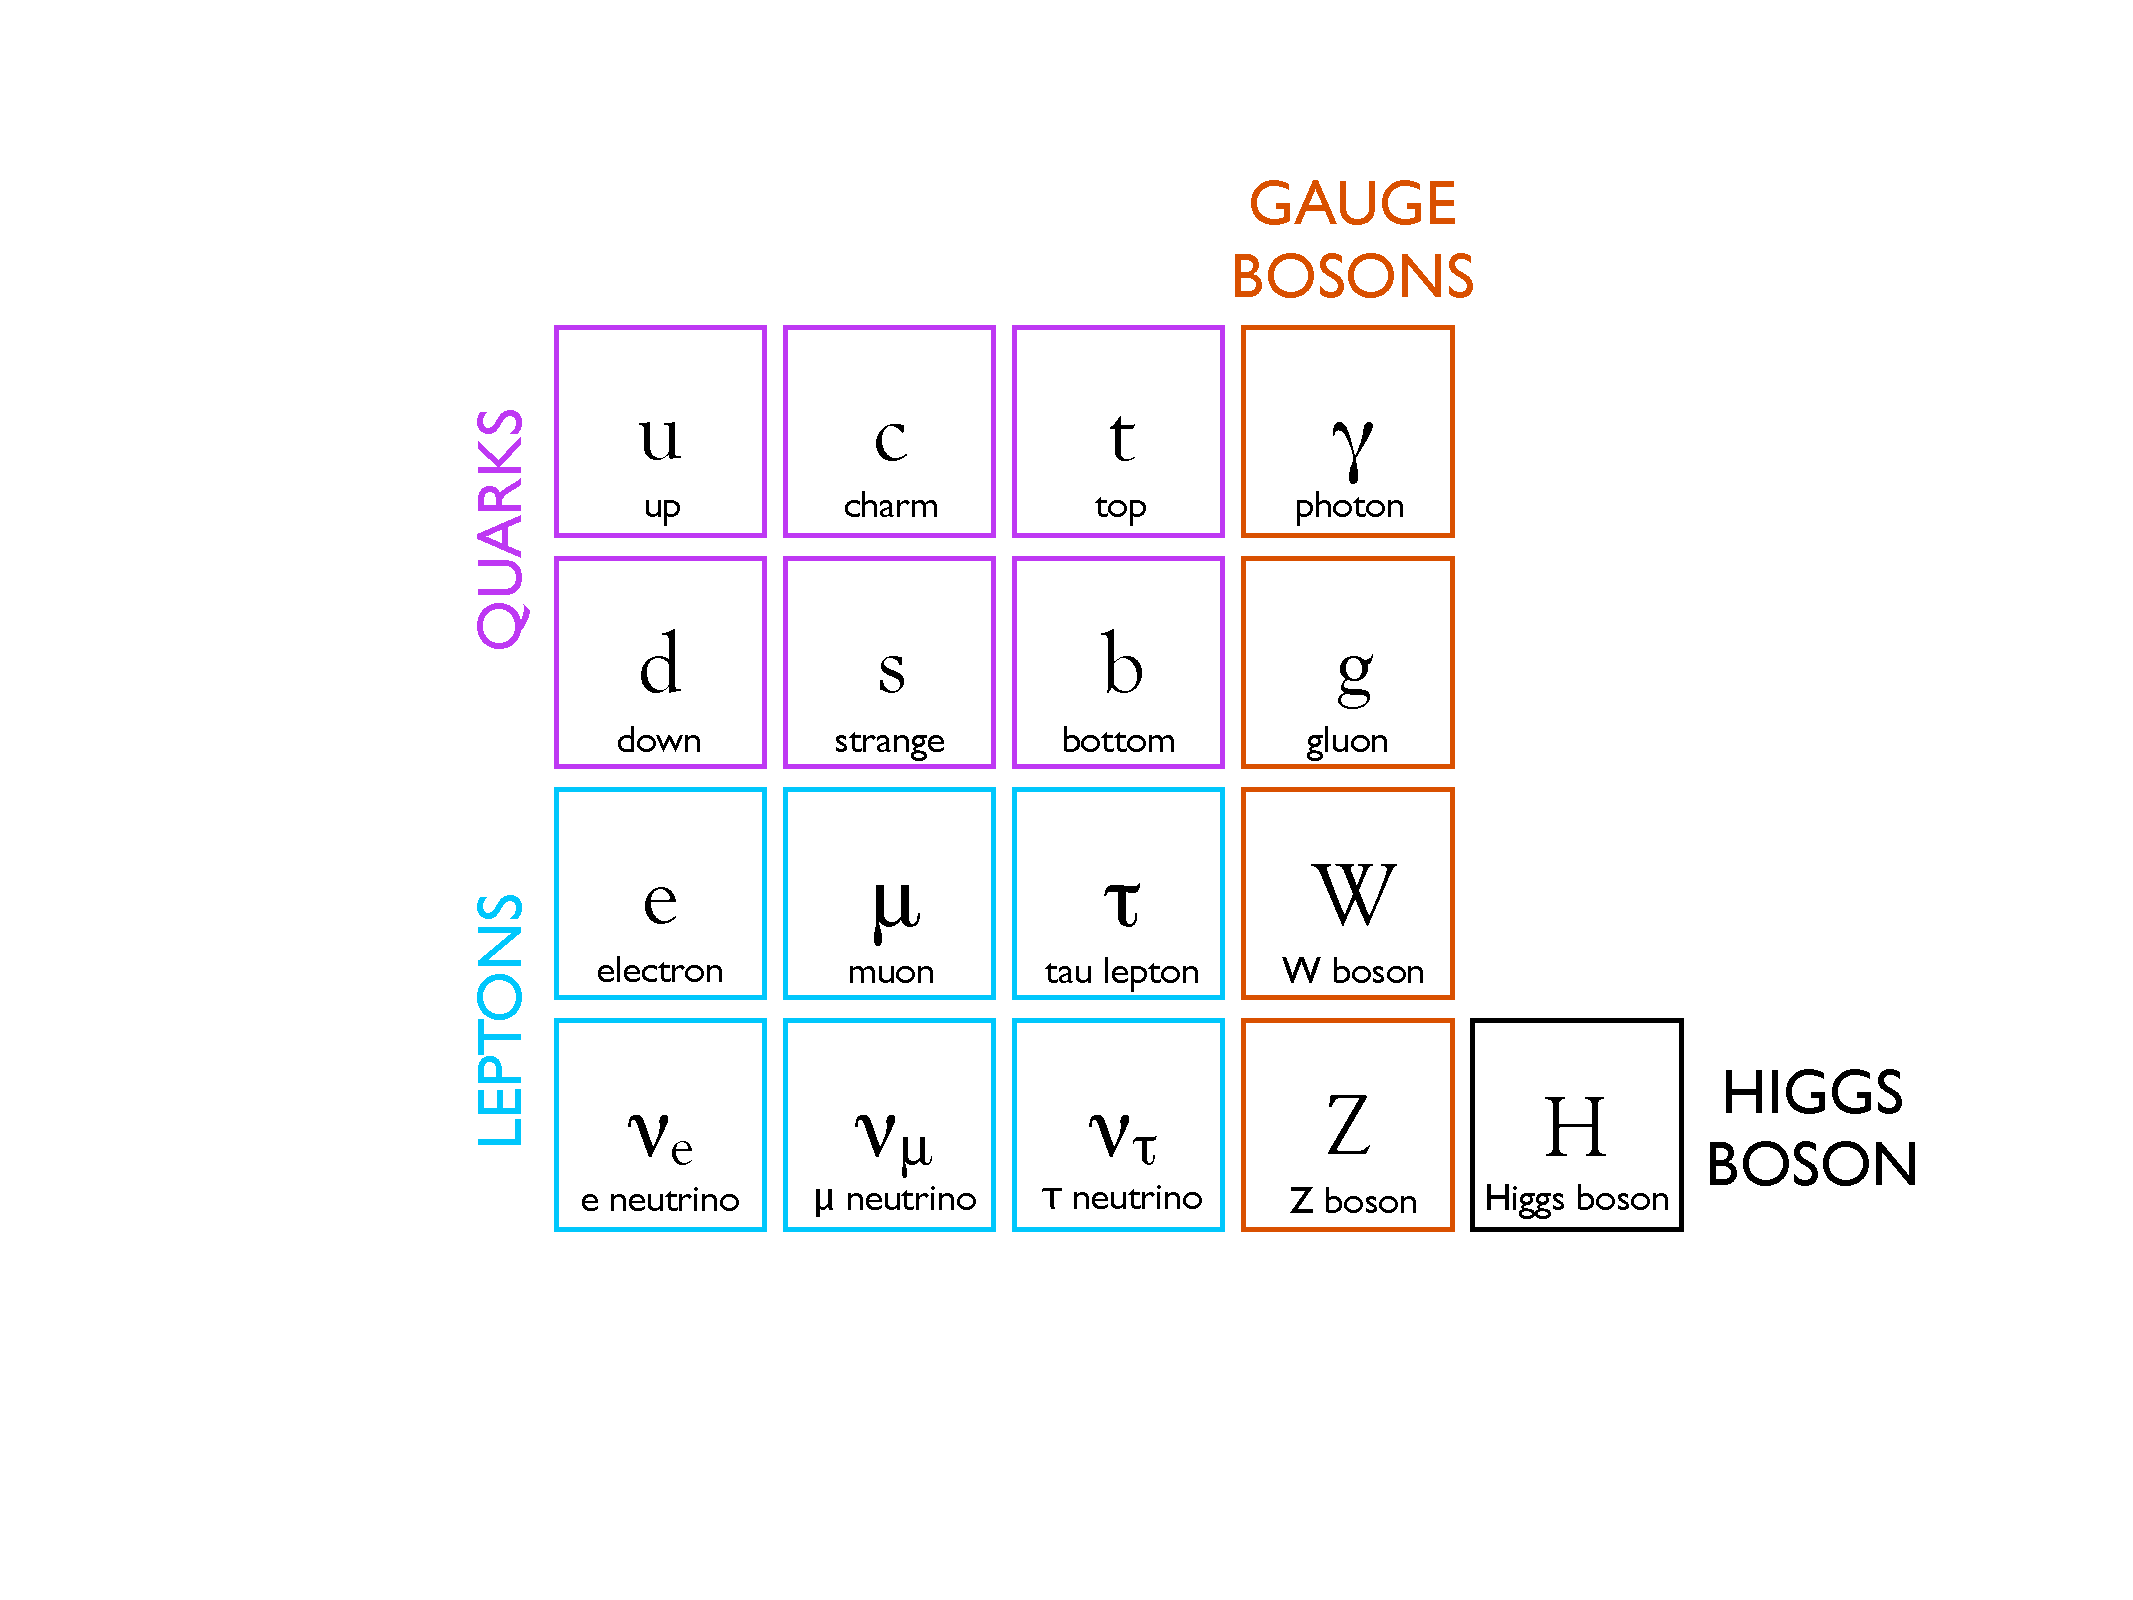
\includegraphics[width=0.6\textwidth]{figures/StandardModelTable}
      \caption{Standard Model particles.}
      \label{fig:StandardModelTable}
   \end{center}
\end{figure}

Leptons and quarks are fermions -- particles with half-integer spin whose dynamics obey the Dirac equation (see Equation~\ref{eq:Dirac}). Leptons fall into three generations called ``flavors", and have electric charge equal to integer multiples of the elementary charge $e =$ 1.6$\cdot$10$^{-19}$ C. The negatively charged leptons are the electron, the muon, and the tau (in increasing order of mass), and each is associated with an extremely light, neutral particle called a neutrino. Quarks have fractional multiples of the elementary electric charge and also possess another quantum property known as ``color" charge, whose implications will be explained shortly. There are three generations of quarks and a total of six different quark flavors (two per generation). For each quark and lepton, there exists an associated antiparticle.

The strong, electromagnetic, and weak interactions occur via the exchange of gauge bosons, which obey Bose-Einstein statistics and have spin 1. Each type of interaction involves the coupling of particles to the gauge field associated with that interaction. The theory describing the strong force is called quantum chromodynamics, or QCD. Quantum electrodynamics (QED) describes the electromagnetic force. At energies above $\mathcal{O}$(100) GeV, the electromagnetic interaction force unifies with the weak force, and the unified force is described by the electroweak theory.

Any particle with electric charge can participate in electromagnetic interactions, which are mediated by electrically neutral, massless photons. The strong force is mediated by gluons, which are colorless, electrically neutral, and massless; only quarks and gluons, which possess nonzero color charge, can participate in strong interactions. $W^{\pm}$ or $Z^{0}$ bosons are the carriers of the weak force, which is responsible for such processes as nuclear decays (they will hence be referred to as $W$ and $Z$, dropping the charge superscript unless it is necessary to mention their charges explicitly). W$^{+}$ and W$^{-}$ are one another's antiparticles, while Z and the photon are their own antiparticles. Unlike the gluon and photon, the $W$ and $Z$ bosons are massive.

The Standard Model belongs to the symmetry group SU(3)$\times$SU(2)$\times$U(1). The QCD Lagrangian $\mathcal{L}_{QCD}$ obeys the symmetry of the special unitary group SU(3), while the electroweak portion $\mathcal{L}_{EWK}$ obeys SU(2)$\times$U(1) symmetry.

In QCD, the eight generators of the SU(3) group give rise to eight gauge fields $G^{a}_{\mu}$, whose linear combinations correspond to gluons. The conserved quantity in QCD interactions is ``color" charge. An unusual feature of the strong force is that as the momentum transfer of the interaction increases, the strength of the interaction decreases. Thus, for high-energy interactions, the QCD coupling is small enough that perturbation theory can be applied to Feynman diagrams and quarks can be treated like free particles -- a property known as asymptotic freedom. The behaviour of the strong force at low energies, where QCD becomes non-perturbative, is still not well understood; one consequence of the low-energy scale behaviour of the strong force is color confinement, which means that quarks and antiquarks cannot be found free but can only exist in bound states called hadrons. The SU(3) invariance of hadronic wavefunctions restricts the only possible hadronic states to be SU(3) singlets -- i.e., states with a net zero color charge.

The quarks that make up a hadron, the gluons that bind them, and the fleeting quark-antiquark pairs that these gluons produce are collectively known as partons. The probability density for each parton to be found with a fraction $x$ of the total hadronic 4-momentum is described by its parton distribution function (PDF), which is determined by the strong interactions among the various partons in the hadron. In practice, PDFs cannot be calculated from theory alone because of the non-perturbative nature of QCD interactions at low energies; thus, they can only be measured experimentally~\cite{BettiniPhysics}.

Low-energy weak processes such as beta decays were first described by Fermi via a simple four-point interaction~\cite{0034-4885-42-12-001}. This, however, does not explain the experimental observation of parity violation in weak decays, and the predicted cross-section for weak decays blows up for high-energy processes ($q^2 >$ $\mathcal{O}$(100 GeV)$^2$) in the four-point interaction model. Electroweak theory developed in response to these issues; it predicted that weak interactions occur via parity-violating axial vector currents mediated by massive vector bosons~\cite{PerkinsPhysics}. In electroweak theory, the gauge fields $B_{\mu}$ (from the U(1) group) and \textbf{W}$^1$$_{\mu}$, \textbf{W}$^2$$_{\mu}$, and \textbf{W}$^3$$_{\mu}$ (from the SU(2) group) give rise to the electroweak gauge bosons~\cite{Bednyakov:2007pz}.

However, a problem arises from the fact that the Lagrangian for the electroweak gauge bosons can only be invariant under SU(2)$\times$U(1) transformations if the masses of its gauge bosons are zero. Although the photon is known to be massless, the $W$ and $Z$ bosons are clearly not. A prediction for the mass of the $W$ was first derived from measurements of the lifetime of the muon~\cite{ThomsonPhysics}, and the $W$ and the $Z$ were later both discovered in e$^{+}$e$^{-}$ collisions in the LEP experiment at CERN~\cite{Arnison:1983rp,Arnison:1983mk}.

\begin{figure}
   \begin{center}
      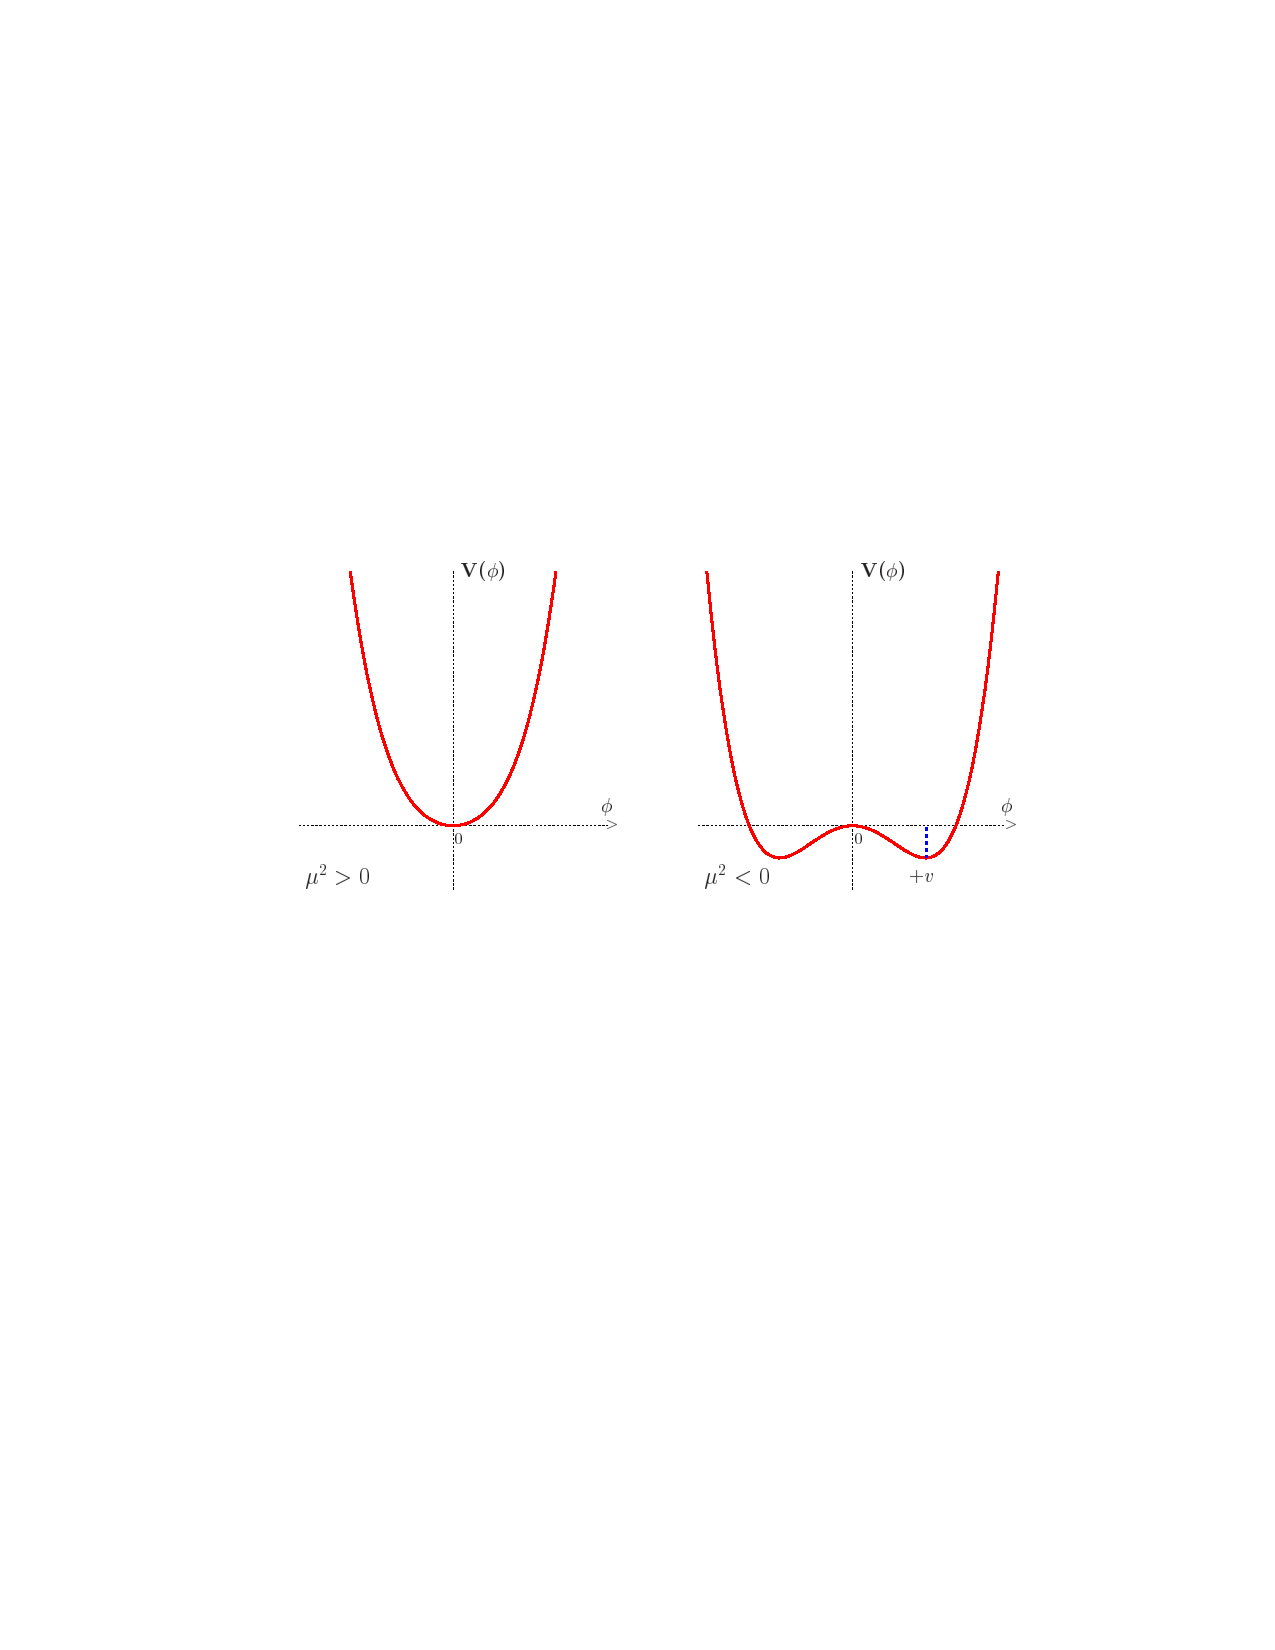
\includegraphics[width=0.6\textwidth]{figures/intro-Higgspotential}
      \caption{Illustration of spontaneous symmetry breaking in the case of a real scalar field $\phi$, with potential V($\phi$) $= \frac{1}{2}\mu^2\phi^2 + \frac{1}{4}\lambda\phi^4$. For $\mu^2 > 0$ (\cmsLeft), the potential has a minimum at zero and thus the vacuum expectation value of the field is zero. For $\mu^2 < 0$ (\cmsRight), the potential has two nonzero minima at $v = \pm\sqrt{-\frac{\mu^2}{\lambda}}$; in nature, the symmetry is broken by the choice of one of these two possible values for the vacuum expectation value of the field. Image copied from~\cite{Djouadi:2005gi}.}
      \label{fig:higgspotential}
   \end{center}
\end{figure}

The massive gauge boson paradox is resolved by the concepts of spontaneous symmetry breaking and the Higgs mechanism~\cite{ThomsonPhysics}. This involves the introduction of a complex scalar field whose vacuum expectation value is not zero but instead one of multiple nonzero minima of the scalar field potential. The choice of one of these vacuum expectation values breaks the symmetry of the scalar potential. This is illustrated in Figure~\ref{fig:higgspotential} for the simplified case of a real scalar potential with two local minima. When the Lagrangian of such a scalar field is expressed in terms of a perturbation of the field about its vacuum expectation value, this results in a mass term for the perturbation that corresponds to a scalar boson called a Goldstone boson.

To complete the picture, the spontaneous symmetry of the scalar field is embedded in the SU(2)$\times$U(1) symmetry, and this results in what is known as the Higgs mechanism. The simplest model requires two complex scalar fields. When the combined Lagrangian of the scalar fields and electroweak gauge fields is expressed as an expansion about the chosen vacuum expectation values of the scalar fields, one ends up with terms quadratic in the $B_{\mu}$, \textbf{W}$^1$$_{\mu}$, \textbf{W}$^2$$_{\mu}$, and \textbf{W}$^3$$_{\mu}$ fields, which are interpreted as mass terms. Via an appropriate gauge transformation, the Goldstone bosons resulting from the symmetry breaking disappear by being absorbed into the longitudinal degree of freedom of the \textbf{W}$^i$$_{\mu}$ fields, and the mixing of the four gauge fields results in the $W^{\pm}$ bosons, which are linear combinations of \textbf{W}$^1$$_{\mu}$ and \textbf{W}$^2$$_{\mu}$, and a $Z$ boson and a photon, both of which are linear combinations of \textbf{W}$^3$$_{\mu}$ and $B_{\mu}$. When this mixing is accounted for in the Lagrangian, the only mass terms that remain are the ones for the $W$ and $Z$ bosons, while the photon is massless. The existence of the Higgs field also generates the masses of the fermions via Yukawa interactions between fermions and the Higgs field in the electroweak Lagrangian.

\begin{figure}
   \begin{center}
      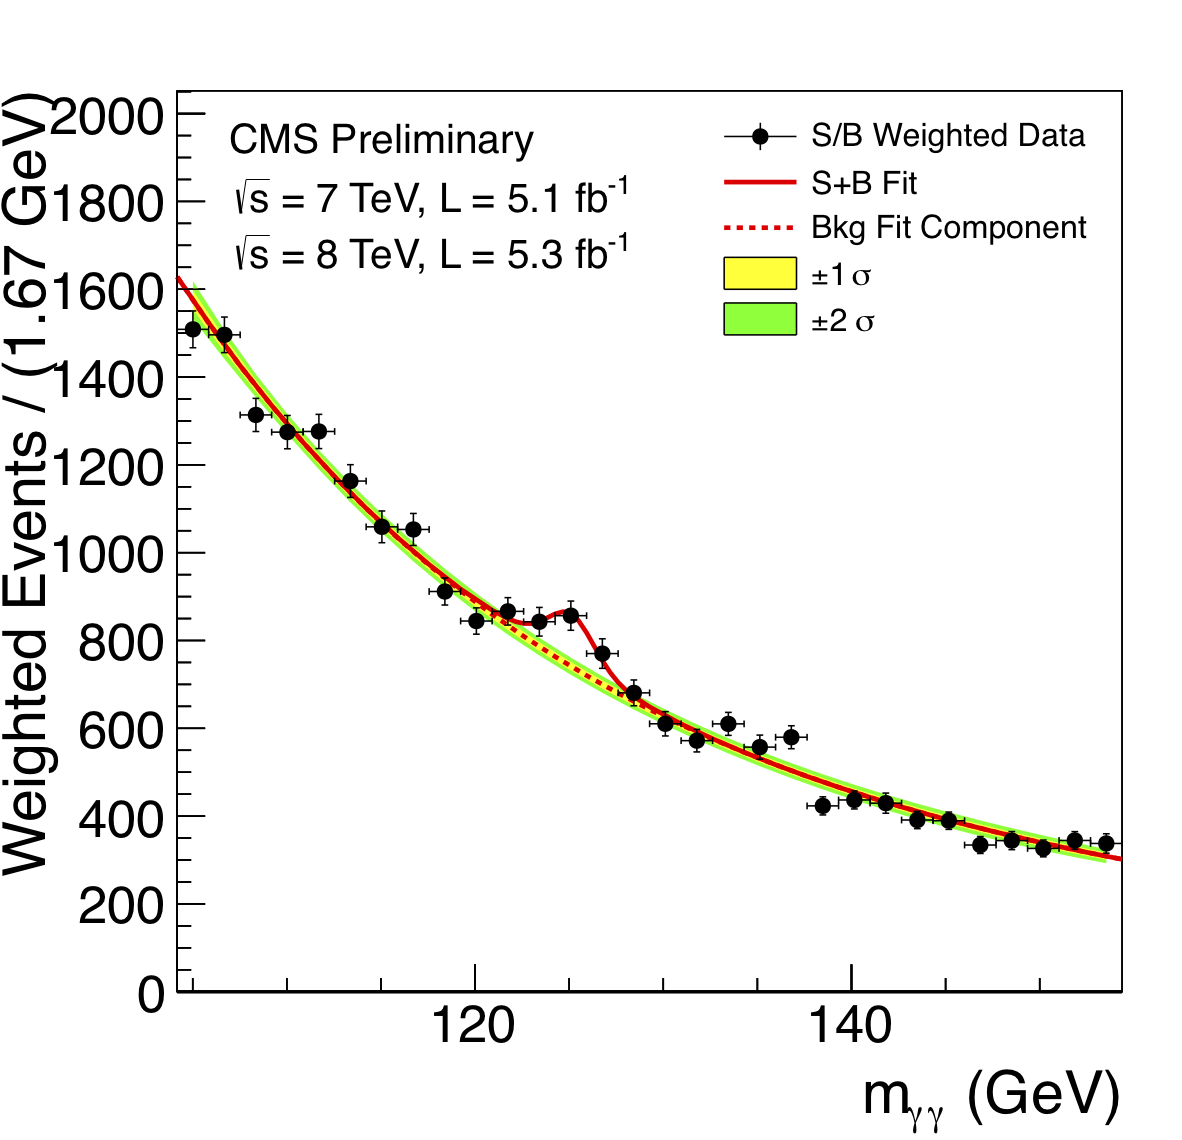
\includegraphics[width=0.6\textwidth]{figures/higgs-resonance}
      \caption{Observation of the Higgs resonance at 125 $\pm$0.4 (stat.) $\pm$0.5 (syst.) GeV in the diphoton spectrum at the CMS experiment~\cite{Chatrchyan:2012ufa}.}
      \label{fig:higgs-resonance}
   \end{center}
\end{figure}

Thus, the electroweak theory predicts the existence of a Higgs boson. This is the final particle is represented in Figure~\ref{fig:StandardModelTable}, the only known scalar particle in the Standard Model. The experimental search for this Higgs boson has carried on for decades after its existence was first predicted, and has finally culminated in its discovery at the LHC collider at CERN~\cite{Aad:2012tfa,Chatrchyan:2012ufa} (see Figure~\ref{fig:higgs-resonance}), providing a strong validation for this last major prediction of the Standard Model.

\section{Deficiencies of the Standard Model\label{sec:SMdeficiencies}}

Although the Standard Model has been successful in describing a wide range of experimental results, there is clear evidence that it is not complete. To name a few of its shortcomings~\cite{BettiniPhysics}:

\begin{itemize}
\item \textbf{Gravity: }The four fundamental forces are the strong force, electromagnetism, the weak force, and gravity. The Standard Model accounts for the first three, but the way in which gravity, which is $10^{32}$ times weaker than the weak force, factors into the Standard Model is still unknown.
\item \textbf{Neutrino oscillations: }The Standard Model treats neutrinos as massless particles. However, there is strong experimental evidence to the contrary. The observation of neutrino flavor oscillations, which cannot occur if neutrinos were massless, suggests that the observed electron, muon, and tau neutrino flavors are not in fact mass eigenstates -- rather, the observed neutrino flavor states are superpositions of mass eigenstates. What the mass eigenvalues are and why they are so small, are mysteries that remain to be resolved.
\item \textbf{Dark matter and energy: }Matter constitutes only about 30\% of the total mass-energy density of the universe; the remainder is comprised of ``dark matter" and ``dark energy", but their exact nature is unknown, and their presence is only deduced indirectly from their gravitational effects, since dark matter does not emit or absorb electromagnetic radiation. Thus, it is suspected that dark matter must be made up of some different type of particle not accounted for by the Standard Model.
\item \textbf{Grand unification: }The running coupling constants of the strong, electromagnetic, and weak interactions generally approach one another at increasingly higher energy scales. This suggests that these three fundamental interactions (and perhaps also gravity) might be manifestations of one unified field theory and thus may unify at some high energy scale; some theories predict this scale to be on the order of 10$^{16}$ GeV.
\item \textbf{The hierarchy problem: }The Standard Model predicts that the mass of the Higgs boson receives loop corrections from leptons, quarks, and whatever other particles may couple to the Higgs. As a result, the Higgs mass would be expected to receive corrections up to the order of the Planck scale ($\mathcal{O}$(10$^{19}$ GeV)) at which gravity becomes significant and the Standard Model of physics no longer holds. The fact that the magnitude of the actual Higgs mass is so much lower than those of the predicted corrections is surprising, as it implies that there must be some mechanism by which these corrections are cancelled. This constitutes what is known as the hierarchy problem of the Standard Model.
\end{itemize}

These deficiencies indicate that there is physics beyond the Standard Model, and that more elements are needed to provide an accurate description of nature.

\section{Supersymmetry}

One theory that has been proposed to address the hierarchy problem is that there exists a certain symmetry -- called supersymmetry -- that relates fermions to bosons~\cite{Martin:1997ns}. For each fermion, there would exist a corresponding bosonic parter particle, and likewise for each boson there would exist a fermionic partner; such partner particles are referred to as superpartners. Under a supersymmetric transformation, a fermion turns into its superpartner and vice versa. Thus, for each loop correction to the Higgs mass, there would be another loop correction from the supersymmetric partner particle; since fermionic loops have a sign opposite that of bosonic loops, the loop corrections would cancel neatly.

As supersymmetry posits a superpartner for every Standard Model particle, it is of great interest to look for experimental evidence of these superpartners, none of which have yet been observed in nature. The question is where to look, since there is nothing that specifies the masses of supersymmetric particles or the other numerous other free parameters in the theory of supersymmetry. These free parameters must be constrained by experimental measurements.

The masses of supersymmetric particles must be different from the masses of their Standard Model counterparts, otherwise the supersymmetric particles would have been observed already. In order to have this inequality in masses, supersymmetry must be a broken symmetry. There are many models for the mechanism of supersymmetry breaking; but in general, in order to achieve the stabilization of the Higgs mass, the symmetry breaking scale is expected to be on the order of 1-10 TeV~\cite{Aitchison:2005cf}. Since the mass splittings between Standard Model particles and their superpartners are determined by the supersymmetry breaking parameters, the masses of the lightest supersymmetric particles are  expected to be around the same scale of 1-10 TeV as well. Thus, if supersymmetric particles exist, it could be possible to discover them in high-energy collider experiments such as the LHC at CERN.

The simplest model incorporating supersymmetry into the Standard Model is the Minimal Supersymmetric Standard Model (MSSM)~\cite{Martin:1997ns}. The details will not be covered here, but the Higgs sector consists of two chiral Higgs supermultiplets $H_u$ and $H_d$, of which the former couples to up-type quarks and the latter couples to down-type quarks and charged leptons. The superpotential $W_{MSSM}$ of the MSSM, which defines the most general non-gauge interactions for the superfields, is:

\begin{equation}
W_{MSSM} = \bar{u}y_{u}QH_{u} - \bar{d}y_{d}QH_{d} - \bar{e}y_{e}LH_{d} + \bar{\mu}H_{u}H_{d}
\label{eq:WMSSM}
\end{equation}

While the MSSM does provide a cancellation of large corrections to the Higgs mass, it comes with deficiencies of its own. One problem, called the $\mu$-problem, stems from the fact that the $\mu$ parameter in Equation~\ref{eq:WMSSM}, which must have the dimension of mass, must be of the order of magnitude of the electroweak scale in order to provide the Higgs doublets with vacuum expectation values on the order of the electroweak scale. However, its magnitude is expected to be more naturally close to the Planck scale, which is significantly larger. Fine-tuning its magnitude to that of the electroweak scale thus seems arbitrary and without theoretical motivation.

The $\mu$-problem is avoided in the Next-to-Minimal Supersymmetric Standard Model (NMSSM)~\cite{Maniatis:2009re}, which extends the Higgs sector of the MSSM by a scalar Higgs singlet field S and ultimately predicts a total of seven Higgs bosons -- a pair of charged ones, three neutral scalars, and two neutral pseudoscalars. The NMSSM superpotential is:

\begin{equation}
W_{NMSSM} = W_{MSSM} + \lambda SH_{u}H_{d} + \frac{1}{3}\kappa S^3 + \frac{1}{2}\mu_{s}S^2
\label{eq:WNMSSM}
\end{equation}

The coupling of the singlet field $S$ to the doublet fields naturally generates an effective $\mu$ term via the expectation value of $S$. Thus, $\mu = \lambda$$<S>$, with the desired magnitude near the electroweak scale. The fact that the NMSSM circumvents the $\mu$-problem makes it of great interest to study. The new physics search presented in this dissertation is a probe into the Higgs sector of the NMSSM.
\chapter{Experiment description\label{sec:experiment}}

\section{Large Hadron Collider\label{sec:lhc}}

The Large Hadron Collider (see~\cite{1748-0221-3-08-S08001} for a detailed description) is a circular accelerator and collider of high-energy particles, straddling the French-Swiss border near Geneva, Switzerland. Constructed between 1998 and 2008, the accelerator consists of 2 rings for counter-circulating proton or ion beams, 27 km in circumference and located at depths as low as 175 m underground in the tunnel previously occupied by the LEP collider ring. Superconducting magnets, composed of NbTi Rutherford conductors cooled to temperatures below 2 K with superfluid helium, generate magnetic fields above 8 T and serve to steer and focus the particle beams (either protons or lead ions) in their trajectory through the accelerator rings.

Protons, derived by ionizing hydrogen gas, are accelerated first via a linear accelerator to an energy of 50 MeV and injected into the Proton Synchrotron Booster, which accelerates them to 1.4 GeV. From there, they are injected into the Proton Synchrotron, which accelerates them further to 25 GeV, and then into the Super Proton Synchrotron, which brings them to an energy of 450 GeV before finally injecting them into the LHC ring, in which they are accelerated to the desired center-of-mass energy for collisions. The LHC has been designed to collide protons at a maximum center-of-mass energy of 14 TeV. During its first run, it operated at center-of-mass energy 7 TeV from 2010-2012, and then at 8 TeV from 2012-2013. After a long shutdown for planned repairs and maintenance, the LHC was restarted in 2015, operating at 13 TeV, with the intention of eventually increasing to 14 TeV.

The LHC is home to several experiments -- the general-purpose high-luminosity detectors ATLAS (A Toroidal LHC Apparatus) and CMS (Compact Muon Solenoid), low-luminosity detectors LHCb (focusing on B physics) and TOTEM (focusing on elastic proton scattering), and the heavy-ion detector ALICE. At each detector, the proton beams are focused together by quadrupole magnets at an interaction point, where they collide, and the particles produced in these collisions are detected and recorded by the detector system. The rest of this chapter will focus on the CMS experiment, where the research described in this thesis was conducted.

\section{Compact Muon Solenoid\label{sec:cms}}

The Compact Muon Solenoid (CMS) detector is a hermetic general-purpose detector at the LHC, gathering data from the collision of proton-proton and heavy ion beams to study a wide range of physics processes. This experiment is characterized by a powerful superconducting solenoid magnet that produces a 4 T magnetic field; the paths of charged particles are bent by the magnetic field, allowing their momenta to be accurately reconstructed from their trajectories. Quadrupole magnets bend the two proton beams passing through the LHC ring to intersect and collide at the interaction point (IP) in the center of the CMS detector, and the particles produced in the collision pass through and are recorded by the layered system of cylindrical subdetectors that comprise the CMS detector. At the center of the ensemble is a silicon tracker subdetector for reconstructing accurately the momenta of charged particles. Encircling it is the electromagnetic calorimeter (ECAL), a homogenous calorimeter that uses scintillating lead tungstate crystals to reconstruct electrons and photons with high energy resolution. Outside the electromagnetic calorimeter is the hadron calorimeter (HCAL), a sampling calorimeter with alternating layers of brass and scintillator that measures the energy deposited in hadronic showers. The solenoid magnet is located outside the hadronic calorimeter, together with an iron yoke system that provides a return flux for the magnetic field. The outermost layer of the CMS detector is the muon tracking system for identifying and reconstructing the trajectories of muons. The solenoid magnet and the various subdetectors of CMS will be described in more detail in the rest of this chapter, followed by considerations regarding the mechanisms for data collection by CMS. A more complete description of the detector can be found at~\cite{1748-0221-3-08-S08004}; unless otherwise specified, all information in this chapter is derived from this source.

\subsection{Magnet\label{sec:cms-magnet}}
% solenoid, yoke, cryogenics, vacuum system

The superconducting solenoid magnet of CMS encloses the tracker detector, ECAL, and part of the HCAL inside a cylindrical bore 6.3 m in diameter and 12.5 m long, weighing 220 tonnes. The solenoid is composed of a 4-layer winding of coils made of NbTi, which is mechanically reinforced by being mixed with an aluminium alloy, an innovative method that makes the coils serve both as conductors and as their own self-stabilizing structural support. At full current, the solenoid carries 19.14 kA, producing a nearly uniform 4 T magnetic field through the volume enclosed by the bore, containing 2.6 GJ of stored energy. The magnetic flux is returned through an iron yoke, consisting of a system of barrel wheels and endcap disks arranged outside the volume of the solenoid in a cylindrical pattern and interleaved with the muon tracking system; the yoke consists of 5 iron rings, each 2.536 m wide in the z direction, positioned at z = -5.342 m, -2.686 m, 0 m, +2.686 m, and +5.342 m (rings number -2, -1, 0, 1, and 2 respectively).

\subsection{Tracker\label{sec:cms-tracker}}

5.8 m in length along the z axis and 2.5 m in diameter, the tracker detector is the innermost layer of the CMS detector system. Its purpose is to reconstruct the paths and momenta of charged particles with transverse momentum 1 GeV and upwards, and to provide good impact parameter resolution for accurately reconstructing the positions of secondary vertices, which are displaced from the point of collision and generally are a characteristic signature of long-lived particles such as those from heavy-flavour processes. Since the tracker detector receives higher irradiation than any other part of the detector due to its proximity to the beam line and the interaction point (IP), the tracker detector has been designed to perform in a high-flux environment, with thousands of particles passing through its volume every 25 ns when the LHC is running at its design luminosity. Thus, the tracker has been designed with these challenges in mind in order to yield good position and time resolution.

The tracker detector is composed of two subdetectors. The one closest to the beam line is the pixel detector; its sensors are 100 $\mu$m x 150 $\mu$m pixels, which receive an occupancy on the order of $10^{-4}$ per pixel per bunch crossing. The second and larger subdetector is the silicon strip tracker, whose sensors are silicon strips; since it is located at larger radii than the pixel detector, the fluence of particles that reach it is lower and thus the granularity of the silicon strips can be considerably lower than that of the pixel detector, with strip areas ranging from 10 cm x 80 $\mu$m at intermediate radii for the inner strip tracker (20 $<$ r $<$ 55 cm) and 25 cm x 180 $\mu$m for the outer strip tracker (55 $<$ r $<$ 110 cm), resulting in an occupancy of about 2-3\% for the inner tracker and 1\% for the outer tracker. In total, the CMS tracker detector is comprised of 200 $m^{2}$ of active silicon sensors, providing a coverage of up to $\abs{\eta}$ $<$ 2.5.

The support structures that hold the sensors in position are designed to minimize the amount of material used, since energy loss via multiple scattering and extraneous particles produced by nuclear interactions, gamma conversions, and bremsstrahlung in the supporting material can all interfere with tracking efficiency. Because of the high particle fluence passing through the tracker volume during operation, radiation-hard sensors and electronics are required to withstand the radiation dosage; also, an efficient system system of cooling tubes carrying chilled liquid $C_{6}F_{14}$ pervades the tracker volume, keeping it at or below -10 C during operation, thus minimizing radiation damage to the sensors caused either by direct irradiation or by the annealing of radiation-induced defects in the silicon crystal structure through thermal agitation.

\subsubsection{Pixel detector\label{sec:cms-pixel}}
% barrel and disks, design of sensors, electronics, readout

The pixel detector is the innermost layer of the tracker detector, with three concentric cylindrical barrel layers complemented by two endcap disks on either side of the interaction point. The barrel layers are located at radii 4.4, 7.3, and 10.2 cm from the beam line, extending out to 2.9 m from the interaction point in the $\pm$z directions. Two endcap disks are located at z $=$ $\pm$34.5 cm and $\pm$46.5 cm, with inner radius 6 cm and outer radius 15 cm. Both the barrel cylinders and endcap disks are split in halves along the y axis for ease of extraction and access. Each sensor has an area of 100 $\mu$m x 150 $\mu$m; the nearly square design is intended to provide good cluster size and hit resolution in both r$\phi$ and z for the barrel and r$\phi$ and r for the endcaps, as both of these coordinates are needed for measuring track impact parameters.

In the barrel, the sensors are arranged 2 x 8 on rectangular modules (or 1 x 8 along the edges of the half-cylinders). In each endcap half-disk, 12 trapezoidal support structures called blades hold the sensors, which come in arrangements of five different plaquette sizes (1 x 2, 2 x 3, 2 x 4, 1 x 5, and 2 x 5) in order to achieve full coverage of the wedge-shaped area of the blade. Altogether, the pixel detector covers a pseudorapidity range of $\abs{\eta}$ $<$ 2.5.

The pixel sensors consist of 52 x 80 high-dose $n$-type pixels implanted in a high-resistance $n$-type substrate of 320 $\mu$m thickness on a sensor plate. Each pixel is bump-bonded onto a readout chip (ROC) connected to the sensor plate. The ROC collects and amplifies the analog signals from the pixels, storing them in a buffer until the arrival of the appropriate readout control and clock signals causes it to pass the sensor signal on to the readout system.
 
When a charged particle passes through a silicon sensor, it induces charge carriers in the n-doped silicon substrate; traveling towards the pixels to be collected, electrons undergo a signficant Lorentz drift (roughly 32$^{\circ}$) due to the 4 T magnetic field along the z axis through the tracker volume, and thus the signal current ends up being spread over adjacent pixels. Interpolation between signals from multiple neighbouring pixels can be used to improve hit resolution. In the barrel, the normal direction of the pixel cells points along the radial direction, perpendicular to the magnetic field, so the Lorentz drift is along the r$\phi$ direction. To induce charge sharing in the pixel endcaps, whose normal points along the magnetic field axis, the blades are rotated at a 20$^{\circ}$ angle about their radial axis in a turbine-like geometry.

\subsubsection{Silicon strip detector\label{sec:cms-strips}}
% barrel and disks, design of sensors, electronics, readout

Outside the pixel detector, at radius 20 cm to 116 cm about the beam line and extending 118 cm in the +z and -z directions, lies the silicon strip detector. It is composed of 3 main subsystems: the tracker inner barrel and disks (TIB and TID), the tracker outer barrel (TOB), and the tracker endcaps (TEC). To optimize coverage, the silicon microstrip sensors in any given barrel layer or endcap disk are positioned to partially overlap with one another, thus resulting in a nonzero pitch with respect to the surface to which they are attached.

The TIB consists of 4 barrel layers 140.0 cm in length, with radii of 255.0 mm, 339.0 mm, 418.5 mm, and 498.0 mm, altogether providing up to 4 r-$\phi$ measurements per particle trajectory. The sensors are silicon microstrips with a thickness of 320 $\mu$m, lying parallel to the beam axis, with a pitch of 80 $\mu$m on the inner two layers and 120 $\mu$m on the outer two layers, yielding a single-point resolution of 23 $\mu$m for the inner two layers and 35 $\mu$m for the outer two layers. The TID is comprised of six endcap disks, three at each end of the TIB between $\pm$80.0 cm and $\pm$90.0 cm on the z axis; each disk consists of three support rings from radius 200 $\mu$m to 500 $\mu$m. Silicon microstrips, similar to the ones used in the barrel, lie radially on the disks, with a pitch varying from 100 $\mu$m to 141 $\mu$m. While the pixel detector is split down the y axis into half-cylinders for ease of installation, access, and independent testing, the TIB and TID are split into half-shells along the x axis for similar reasons. Two carbon-fibre service cylinders are coupled to the $\pm$z ends of the TIB, providing a route to the TIB shells for service cables originating from a service distribution disk called a margherita, and also housing the TID.

The TOB surrounds the TIB with 6 barrel layers, reaching to an outer radius of 116 cm and spanning 118 cm in the $\pm$z directions. The silicon microstrip sensors here are 500 $\mu$m thick and have a pitch of 183 $\mu$m in the inner four layers and 122 $\mu$m in the outer two layers, yielding a single-point resolution of 53 $\mu$m and 35 $\mu$m respectively in those layers. On either end of the TOB, the TEC extends radially from 220 mm to 1135 mm and in the $\pm$z direction from $\pm$1240 mm to $\pm$2800 mm; each side consists of an assembly of 9 disks with up to 7 rings bearing silicon microstrip sensors, plus 2 extra disks that serve as front-back termination. The microstrip sensors used here have a thickness of 320 $\mu$m in the four rings closest to the TOB and 500 $\mu$m in the remaining outer rings, with a pitch varying from 97 to 184 $\mu$m.

The silicon microstrip sensors used have a single-sided p-on-n design. Signal currents are amplified and stored by a custom integrated circuit called an APV25 before being transmitted via optical fibers through the readout system for digitization and storage.

\subsection{Electromagnetic calorimeter\label{sec:cms-ecal}}
% crystals, photodetectors, readout, preshower

The electromagnetic calorimeter (ECAL) is a hermetic homogeneous calorimeter made up of lead tungstate (PbWO$_4$) crystals; similar to the inner tracking system, it is composed of a cylindrical barrel system (with a total of 61,200 crystals) and an endcap system (one endcap disk on each side of the barrel, with 7324 crystals per disk). When electrons or photons pass through the ECAL, the resulting electromagnetic showers that they generate excite the scintillator atoms, causing them to emit blue-green scintillation light (up to 420-430 nm in wavelength) that is collected, amplified, and read out by photodetectors glued to the ends of the crystals. High granularity is needed for good energy resolution in the ECAL; the choice of PbWO$_4$, with a density of 8.28 g/cm$^3$, a radiation length of 0.89 cm, and a Moliere radius of 2.2 cm, allows for compact, granular crystals that can resist radiation damage under the high particle fluences that the detector is subjected to throughout its operation. As the number of scintillation photons produced by the crystals and the amplification provided by the photodiodes both tend to decrease with increasing temperature, the temperature of the ECAL detector needs to be maintained at a steady operating temperature during its operation; this is done by a cooling system that uses water as a coolant, maintaining the ECAL at a stable temperature of 18$^{\circ}$ C with an uncertainty of $\pm$0.05$^{\circ}$ C.

The barrel extends from an inner radius of 1.29 m to an outer radius of 1.77 m. In the barrel, the detector granularity is 360-fold in $\phi$ and 170-fold in $\eta$. The crystals have a truncated pyramidal shape that varies with their position in $\eta$, with a cross-sectional area of approximately 22x22 mm$^2$ at the front face (closest to the beam line) and 26x26 mm$^2$ at the rear face, and a length of 230 mm (corresponding to 25.8 radiation lengths). Groups of 2x5 barrel modules are referred to as sub-modules, encased within a 0.1-mm thick wall consisting of an aluminium layer facing the crystal, followed by two layers of glass fibre-epoxy resin. Submodules are grouped together into larger groups called modules containing 400 or 500 crystals, whose shape depends on the position in $\eta$ of the module. Four modules form a supermodule, and 18 supermodules form half a barrel.

On either side of the barrel, the ECAL endcaps cover the pseudorapidity range 1.479 $<$ $\abs{\eta}$ $<$ 3.0. Endcap crystals have a truncated pyramidal shape similar to barrel crystals, with a front face cross-sectional area of about 28.62x28.62 mm$^2$ and a rear face cross-sectional area of 30z30 mm$^2$, and a length of 220 mm (24.7 radiation lengths). They are arranged in groups of 5x5 known as supercrystals, enclosed in a carbon-fibre alveolar wall. Each half of an endcap disk, called a Dee, is composed of 138 full supercrystals and 18 partial supercrystals.

Sandwiched between the barrel and each endcap disk is a disk-shaped sampling calorimeter with a thickness of 20 cm; these two disks make up the preshower detector. Its main purposes are neutral pion identification and rejection in the fiducial region 1.653 $<$ $\abs{\eta}$ $<$ 2.6, identify electrons against the background of minimum ionizing particles, and improve the position resolution of electrons and photons in the ECAL. The preshower is two layers thick; each layer consists of a layer of lead radiators for initiating electromagnetic showers, followed by a layer of silicon strip sensors for detecting the showers.

To take advantage of total internal reflection for the collection of scintillation light, all the ECAL crystals have been precisely polished during production. The crystals have a truncated pyramidal shape, which would tend to cause nonuniform light collection along the length of barrel crystals; thus, in the barrel crystals, one crystal face is left unpolished to compensate for this effect. This technique is not used in the endcaps because the endcap crystal faces are nearly parallel to one another, thus resulting in more uniform light collection. The different magnetic field configuration and particle flux in the barrel and endcaps led to different choices of photodetectors for those two systems: avalanche photodiodes (APDs) for the barrel and vacuum phototriodes (VPTs) in the endcaps. At 18$^{\circ}$ C, approximately 4.5 photoelectrons per MeV of deposited energy are collected by both APDs and VPTs. For electron or photon energies below 500 GeV, the ECAL energy resolution can be estimated as follows:

\begin{equation}
(\frac{\sigma}{E})^2 = (\frac{S}{\sqrt{E}})^2 + (\frac{N}{E})^2 + C^2
\end{equation}

In this equation, S is the stochastic term, N is the noise term, and C is the constant term. The stochastic term S comes from stochastic fluctuations in electromagnetic shower containment, a photostatistics contribution of 2.1\% coming from the uncertainty on the number of primary photoelectrons produced per MeV of deposited energy, and fluctuations in the energy deposited in the preshower absorber. The term N accounts for noise due to electronics, the signal digitization process, and energy deposited by pileup particles. Finally, the constant term C covers various sources of systematic error including the nonuniformity of light collection due to crystal shape, intercalibration errors, and leakage of energy from the back of the crystal.

\subsection{Hadronic calorimeter\label{sec:cms-hcal}}
% HB, HE, HO, HF -- scintillator, absorber, readout

Surrounding the ECAL is the hadronic calorimeter (HCAL), a sampling calorimeter extending radially from 1.77 m to 2.95 m from the beam line. Its main goals are to measure the energy deposited by hadronic jets in each event, and to measure indirectly the missing energy due to neutrinos and any potential exotic particles. The HCAL is split up into four subsystems, of which the innermost are the HCAL barrel and endcaps. To provide enough calorimeter material to absorb hadronic showers for jet and missing energy measurement while respecting the spatial constraints from ECAL within and the superconducting solenoid without, the barrel and endcaps are supplemented respectively by the outer calorimeter outside the solenoid and the forward calorimeters outside the muon endcaps. Altogether, these four subsystems provide coverage up to $\abs{\eta}$ $<$ 5.2.

The barrel system (HB) covers up to $\abs{\eta}$ $<$ 1.3. It is subdivided transversally into two half-barrels, each of which consists of 18 identical wedges (making a total of 36 HB wedges). The wedges are subdivided into 4 azimuthal sectors staggered for optimum coverage, and they hold the absorber plates and scintillator material. The HB absorber is made up of an innermost 40-mm-thick steel front plate, eight 50.5-mm-thick brass plates, six 56.5-mm brass plates, and an outermost 75-mm-thick steel back plate. Passing hadrons interact with the nuclei of the absorber, producing hadronic showers of quarks and gluons. The energy in these showers is deposited in and measured by 17 layers of scintillator material that are interspersed between the absorber plates; layers in azimuthal sectors 1 and 4 fit into slots in the edges of a wedge, while layers in azimuthal sectors 2 and 3 fit into slots in the middle of a wedge. Besides the division into 18 sectors in $\phi$, the scintillator material is also split into 16 sectors in $\eta$, resulting in a granularity of (0.087, 0.087) in ($\eta$, $\phi$).

The smallest scintillator unit is called a tile; tiles in layer 0 are made of Bicron BC408 and primarily serve to sample hadronic showers that develop between the HB and the ECAL barrel, while tiles in layers 1-16 are made of of Kuraray SCSN81 plastic scintillator. Tiles in a given azimuthal layer are grouped into units called trays for ease of assembly, access, and individual testing; each barrel layer contains a total of 108 trays. The scintillation light produced in each tile is collected by a Kuraray Y-11 wavelength-shifting (WLS) fibre. Each WLS fibre is spliced to a clear Kuraray double-clad fibre that serves all the tiles in the tray and delivers the collected light to an optical decoding unit, which arranges the clear fibres into readout towers and transmits their signals to a hybrid photodiode (HPD) for amplification and readout. Multipixel HPD's were chosen because of the wider range of wavelengths that they can detect and their low sensitivity to magnetic fields; those used in the HB, HE, and HO have a gain of ~2000.

The endcap system (HE) disks on either side of the HB are mounted onto the iron yoke of the muon endcap system and span the pseudorapidity range 1.3 $<$ $\abs{\eta}$ $<$ 3. The HE disks are subdivided azimuthally into 36 identical wedges and 18 layers, with 79-mm-thick brass absorber plates. The active material in the trapezoidal scintillator tiles is Bicron BC408 for layer 0 and SCSN81 for the remaining 17 layers. The HE contains a total of 20916 tiles, arranged into 1368 trays, with a granularity of (0.087, 0.087) in ($\eta$, $\phi$) for $\abs{\eta}$ <$\textless$1.6 and (0.087, 0.087) for $\abs{\eta}$ $\geq$ 1.6. The collection of scintillation light by WLS fibres and the transmission of the collected signal from tray to HPD for readout is similar to the design of the HB.

The cylindrical outer calorimeter (HO) is located outside the solenoid, taking advantage of the solenoid coil as an additional sampling layer for late-starting hadronic showers. The HO layers are mounted within the iron yoke that returns the magnetic field of the solenoid; they are the first sensitive layer in each of the 5 rings of the yoke. Ring 0 of the yoke has two layers of HO scintillators on either side of a 19.5-cm thick iron barrel at radii 3.82 and 4.07 m, while the other four rings have one layer of HO scintillator at radius 4.07 m. Each layer of the HO is divided into 12 sectors in $\phi$, each separated by the dead space of 75-mm-thick steel beams that are part of the support structure of the return yoke and the muon system. The HO layers are 40 mm thick, of which 16 mm corresponds to the detector layer and the rest is occupied by aluminium support structures. The tiles in the HO are grouped into towers with a granularity of (0.087, 0.087) in ($\eta$, $\phi$) and have a similar WLS scintillation light collection and HPD readout to the HE and HB trays. Each HO tray spans 5$^{\circ}$ in $\phi$ and the entire range of a muon ring in $\eta$. Studies done to assess the effect of the HO on pion energy measurement by the HCAL show that the inclusion of energy measurements in the HO significantly recovers the effects of hadronic shower energy leakage, which thus directly improves the accuracy of missing transverse energy (MET) measurement in an event.

The forward calorimeters (HF)  are located far down the beamline, with the front face of each cylinder at 11.2 m from the interaction point of the CMS detector. The inner radius is 12.5 cm from the beam line, and the outer radius is at 130 cm. Unlike the HB, HE, and HO, the HF calorimeters use quartz fibres rather than plastic as the scintillation medium, so as to withstand the heavy particle fluxes (an average deposited energy of 760 GeV per proton-proton interaction, compared with ~100 GeV for the rest of the HCAL) in the forward region that they occupy. Each HF cylinder is divided azimuthally into eighteen 20$^{\circ}$ wedges; the absorber is composed of 5-mm-thick steel plates with grooves into which the scintillation fibres are inserted. The absorber is subdivided into two parts in $\eta$; in one half, the fibres run through the full depth of the absorber, while in the other half, the fibres start at a depth of 22 cm from the front of the detector. With this design, the HF can distinguish between electromagnetic and hadronic showers, since the former tend to deposit most of their energy within the first 22 cm and the latter deposit nearly equal energy in both segments. 

The quartz fibres are made of a fused-silica core with polymer hard-cladding. Charged particles passing through the crystals with energy above the Cherenkov threshold (roughly 190 keV for electrons) will generate Cherenkov radiation, which constitutes the signal detected; thus, the HF fibres are sensitive to the electromagnetic portion of a hadron shower and are mostly insensitive to neutral hadrons. The fraction of light $f_{trap}$ captured by a crystal is equal to NA/2n$_{core}^2$, where NA is the numerical aperture and n$_{core}$ is the refractive index of the quartz core. The light that hits the core-cladding interface at an angle larger than the critical angle of 71$^{\circ}$ can contribute to the calorimeter signal, while the rest is lost. The fibres run in bundles parallel to the beam line, forming towers with a granularity of (0.175, 0.175) in ($\eta$, $\phi$). Bundles of fibres emerging from the back of the calorimeter are routed to air-core light guides protected by a shielding matrix of steel, lead, and polyethylene. The interior of a light guide is coated with highly reflective metal and guides light to a photomultiplier for readout; one readout box holds 24 photomultipliers and services half of a wedge.

In addition to contributing to hadronic shower energy measurement, the HF is also used to monitor the luminosity of the LHC. The average number of empty towers in the HF is related to the mean number of interactions per bunch crossing, and there is also a linear relationship between luminosity and the average transverse energy per tower.

\subsection{Muon system\label{sec:cms-muon}}
% DT, CSC, RPC, readouts for all

\section{Triggering and data acquisition\label{sec:cms-triggerdaq}}
% rationale, L1, HLT; muon, calorimeter, global

\subsection{Event reconstruction\label{sec:cms-reco}}
% Particle Flow (list all types of particles, focus on muons, taus, jets, MET)
%\include{search-strategy}
%event selection and its rationale
%\include{background-modelling}
% bkg modelling, rationale, and validation
%\include{results and interpretation}
% observed data vs expectation, limits (incl. explanation of CLs)

\bibliography{mythesis}

% The UMI abstract uses square brackets!
\UMIabstract[The abstract that is submitted to UMI must be formatted as shown in the example here. The body of the abstract cannot exceed 350 words. It should be in typewritten form, double-spaced, and on bond paper. It is important to write an abstract that gives a clear description of the content and major divisions of the dissertation, since UMI will publish the abstract exactly as submitted. Students completing their requirements under Plan A should provide extra copies of the typed summary for use by the dissertation committee during the examination.

The abstract that is submitted to UMI must be formatted as shown in the example here. The body of the abstract cannot exceed 350 words. It should be in typewritten form, double-spaced, and on bond paper. It is important to write an abstract that gives a clear description of the content and major divisions of the dissertation, since UMI will publish the abstract exactly as submitted. Students completing their requirements under Plan A should provide extra copies of the typed summary for use by the dissertation committee during the examination.

The abstract that is submitted to UMI must be formatted as shown in the example here. The body of the abstract cannot exceed 350 words. It should be in typewritten form, double-spaced, and on bond paper. It is important to write an abstract that gives a clear description of the content and major divisions of the dissertation, since UMI will publish the abstract exactly as submitted. Students completing their requirements under Plan A should provide extra copies of the typed summary for use by the dissertation committee during the examination.

The abstract that is submitted to UMI must be formatted as shown in the example here. The body of the abstract cannot exceed 350 words. It should be in typewritten form, double-spaced, and on bond paper. It is important to write an abstract that gives a clear description of the content and major divisions of the dissertation, since UMI will publish the abstract exactly as submitted. Students completing their requirements under Plan A should provide extra copies of the typed summary for use by the dissertation committee during the examination.]

\end{document}
